% AMRITA UNIVERSITY B.TECH THESIS TEMPLATE - AIDS TEAM 14 %
\documentclass[a4paper, 12pt]{report}
\usepackage[margin=0.8in]{geometry}
\usepackage{bold-extra}
\usepackage{amsmath}
\usepackage{amsfonts}
\usepackage{amssymb}
\usepackage{graphicx}
\usepackage[english]{babel}
\usepackage[autostyle, english=american]{csquotes}
\MakeOuterQuote{"}
\usepackage{setspace}
\onehalfspacing
\usepackage{amsthm}
\usepackage{array}
\usepackage{cite}
\usepackage{longtable}
\usepackage{fancyhdr}
\usepackage{titletoc}
\usepackage{booktabs}
\usepackage{xcolor}
\theoremstyle{definition}
\newtheorem{Definition}{Definition}[section]

%-------------------------------------------------------------
% Title Page
\begin{document}
	\pagenumbering{gobble}
	\thispagestyle{empty}
	\begin{large}
		\begin{center}
			{\Large\bfseries{REAL-TIME TOPOGRAPHIC ANOMALY DETECTION AND STATEFUL SEMANTIC GUARDRAILS IN HIGH-DIMENSIONAL EMBEDDING SPACES FOR SECURE AGENTIC RAG}}\\
			\vspace{1.0cm}
			A Project Thesis \\
			\vspace{.1cm}
			Submitted in partial fulfilment for the Degree of\\
			\vspace{.1cm}
			BACHELOR OF TECHNOLOGY\\
			\vspace{.1cm}
            in \\
            ARTIFICIAL INTELLIGENCE AND DATA SCIENCE \\
			\vspace{0.8cm}
			by\\ \vspace{0.2cm}
			{\large\bfseries{VIGNESH V S (cb.ai.u4aid23057)}} \\ 
            {\large\bfseries{KARTHICK RUBAN T (cb.ai.u4aid23017)}} \\
            {\large\bfseries{SANJAY SENTHIL (cb.ai.u4aid23042)}} \\
            {\large\bfseries{HARI PRAKASH V (cb.ai.u4aid23047)}} \\
            \vspace{1.5cm}
			
			
\includegraphics[scale=0.65]{univA.png}\\
			\vfill
			DEPARTMENT OF ARTIFICIAL INTELLIGENCE\\
			\Large{\textbf{AMRITA VISHWA VIDYAPEETHAM}}\\
			{\large COIMBATORE CAMPUS (INDIA)}\\
			\vspace*{.3cm}
			October 2026
		\end{center}
	\end{large}

	%------------------------------------------------------------------------------------
	% Bonafide Certificate
	\newpage
	\begin{center}
		{\large DEPARTMENT OF ARTIFICIAL INTELLIGENCE}\\
		\Large{ \textbf{AMRITA VISHWA VIDYAPEETHAM}}\\
		{\large COIMBATORE CAMPUS}\\
		\vspace*{1.5cm}
		
\includegraphics[scale=0.65]{univA.png}\\
		\vspace*{1.0cm}
		{\Large \textbf{BONAFIDE CERTIFICATE}}
	\end{center}
	\vspace*{.5cm}
	\noindent This is to certify that the project thesis entitled \enquote{\textbf{Real-Time Topographic Anomaly Detection and Stateful Semantic Guardrails in High-Dimensional Embedding Spaces for Secure Agentic RAG}} submitted by \textbf{Vignesh V S (Reg. No: cb.ai.u4aid23057)}, \textbf{Karthick Ruban T (Reg. No: cb.ai.u4aid23017)}, \textbf{Sanjay Senthil (Reg. No: cb.ai.u4aid23042)} and \textbf{Hari Prakash V (Reg. No: cb.ai.u4aid23047)} for the award of the \textbf{Degree of Bachelor of Technology} in \textbf{Artificial Intelligence and Data Science} under the \textbf{Faculty of Engineering} is a bonafide record of the work carried out by them under my guidance and supervision at the Department of Artificial Intelligence, Amrita Vishwa Vidyapeetham, Coimbatore Campus.\\
	
    \vfill
    Submitted for the examination held on \dots\dots\dots\dots\dots\dots\dots\dots
    \vfill
    \noindent \textbf{INTERNAL EXAMINER} \hfill \textbf{EXTERNAL EXAMINER}
    \vfill
\begin{center}
	\textbf{Dr. Lekshmi C. R.}\\
	Thesis Advisor \& Project Supervisor,\\
	Assistant Professor,\\
	Department of Artificial Intelligence,\\
	Amrita Vishwa Vidyapeetham,\\
	Coimbatore Campus, India.
\end{center}

	%-------------------------------------------------------------------------------
	% Declaration Page
	\newpage
	\begin{center}
	{\large DEPARTMENT OF ARTIFICIAL INTELLIGENCE}\\
	\Large{ \textbf{AMRITA VISHWA VIDYAPEETHAM}}\\
	{\large COIMBATORE CAMPUS}\\
	\vspace*{2.0cm}
	\large {\textbf{DECLARATION}}
	\vspace*{.3cm}
	\end{center}
	
	\noindent We, \textbf{Vignesh V S} (Reg. No: cb.ai.u4aid23057), \textbf{Karthick Ruban T} (Reg. No: cb.ai.u4aid23017), \textbf{Sanjay Senthil} (Reg. No: cb.ai.u4aid23042) and \textbf{Hari Prakash V} (Reg. No: cb.ai.u4aid23047) hereby declare that this thesis entitled \enquote{\textbf{Real-Time Topographic Anomaly Detection and Stateful Semantic Guardrails in High-Dimensional Embedding Spaces for Secure Agentic RAG}} is the record of original work done by us under the guidance of \textbf{Dr. Lekshmi C. R.}, Assistant Professor, Department of Artificial Intelligence, Amrita Vishwa Vidyapeetham, Coimbatore Campus. To the best of our knowledge, this work has not formed the basis for the award of any degree, diploma, associateship, fellowship, or other similar title to any candidate in any University.\\\\
	
	\vspace*{1cm}
	\noindent{\bf Place: Coimbatore \hfill Signature of the Students} \\
	\noindent {\bf Date: 25-10-2026}
	\vfill
	\begin{center}
		\large{COUNTERSIGNED}\\
	\end{center}
	\vspace{0.4in}
	
\begin{center}
	\textbf{Dr. K. P. Soman}\\
	Professor and Dean, \\ 
	School of Artificial Intelligence, \\ 
	Amrita Vishwa Vidyapeetham,\\
	Coimbatore Campus, India.
\end{center}
	
	%-----------------------------------------------------------------------------
	\clearpage
	\pagenumbering{roman}
	\tableofcontents
	
	\chapter*{Acknowledgements}
	\addcontentsline{toc}{chapter}{Acknowledgements}	
	We express our deep sense of gratitude and sincere indebtedness to our esteemed project supervisor, \textbf{Dr. Lekshmi C. R.}, Assistant Professor, Department of Artificial Intelligence, for her insightful mentorship, technical foresight, and constant encouragement throughout this research. Her critical evaluation and guidance in mathematical formulations and system modeling significantly elevated the quality of this work.
	
	We extend our profound respects to \textbf{Dr. K. P. Soman}, Professor and Dean, School of Artificial Intelligence, for fostering an exceptional research ecosystem and providing access to high-performance computing infrastructure, including NVIDIA A100 GPU clusters.
	
	We also thank all faculty members, technical laboratory coordinators, and our peers at Amrita Vishwa Vidyapeetham, Coimbatore, for their direct and indirect support during the design, implementation, and empirical validation of Vector-Shield.
	\vspace{1cm}
	\begin{flushright}
		\textbf{VIGNESH V S (cb.ai.u4aid23057)}\\
		\textbf{KARTHICK RUBAN T (cb.ai.u4aid23017)}\\
		\textbf{SANJAY SENTHIL (cb.ai.u4aid23042)}\\
		\textbf{HARI PRAKASH V (cb.ai.u4aid23047)}
	\end{flushright}

	\listoffigures
	\addcontentsline{toc}{chapter}{List of figures}
	\listoftables
	\addcontentsline{toc}{chapter}{List of tables}
	\newpage

\section*{{\huge Abbreviations}\hfill} \addcontentsline{toc}{chapter}{\textbf{Abbreviations}}
\vspace{1.2cm}
\begin{tabular}{lll}
RAG ~~~~&--&~~~~ Retrieval-Augmented Generation \\
IPI ~~~~&--&~~~~ Indirect Prompt Injection \\
LOF ~~~~&--&~~~~ Local Outlier Factor \\
PCA ~~~~&--&~~~~ Principal Component Analysis \\
k-NN ~~~~&--&~~~~ k-Nearest Neighbors \\
LLM ~~~~&--&~~~~ Large Language Model \\
SIEM ~~~~&--&~~~~ Security Information and Event Management \\
NLP ~~~~&--&~~~~ Natural Language Processing \\
FP16 ~~~~&--&~~~~ Half-Precision Floating Point (16-bit) \\
BERT ~~~~&--&~~~~ Bidirectional Encoder Representations from Transformers \\
MTEB ~~~~&--&~~~~ Massive Text Embedding Benchmark \\
SOC ~~~~&--&~~~~ Security Operations Center \\
\end{tabular}	
\newpage

\section*{{\huge List of symbols}\hfill} \addcontentsline{toc}{chapter}{\textbf{List of symbols}}
\vspace{1.2cm}
\begin{tabular}{lll}
$\mathbf{v}_i \in \mathbb{R}^d$ ~~~~&--&~~~~ High-dimensional embedding vector of document chunk $i$ \\
$\mathcal{D}_{clean}$ ~~~~&--&~~~~ Manifold of authenticated enterprise clean document vectors \\
$d(\mathbf{p}, \mathbf{q})$ ~~~~&--&~~~~ Cosine distance metric between vectors $\mathbf{p}$ and $\mathbf{q}$ \\
$N_k(\mathbf{p})$ ~~~~&--&~~~~ $k$-nearest neighborhood set of point $\mathbf{p}$ \\
$k\text{-distance}(\mathbf{p})$ ~~~~&--&~~~~ Distance from $\mathbf{p}$ to its $k$-th nearest neighbor \\
$\text{reach-dist}_k(\mathbf{p}, \mathbf{o})$ ~~~~&--&~~~~ Reachability distance between point $\mathbf{p}$ and object $\mathbf{o}$ \\
$\text{lrd}_k(\mathbf{p})$ ~~~~&--&~~~~ Local reachability density of point $\mathbf{p}$ \\
$\text{LOF}_k(\mathbf{p})$ ~~~~&--&~~~~ Local Outlier Factor score of point $\mathbf{p}$ \\
$\tau_{safe}$ ~~~~&--&~~~~ Safe threshold ceiling for Stage 1 pass-through ($\tau_{safe} = 1.30$) \\
$\tau_{anom}$ ~~~~&--&~~~~ Outlier threshold floor for Stage 1 quarantine ($\tau_{anom} = 2.50$) \\
$\mathcal{G} = (\mathcal{V}, \mathcal{E})$ ~~~~&--&~~~~ Stateful cyclic computational graph in LangGraph \\
\end{tabular}
\newpage

\chapter*{Abstract}
\addcontentsline{toc}{chapter}{Abstract}
Enterprise deployment of Autonomous Agentic Retrieval-Augmented Generation (RAG) is critically vulnerable to \textit{Indirect Prompt Injection} (IPI) and vector store poisoning attacks. In these threat models, adversaries embed obfuscated jailbreak instructions within third-party documents (invoices, compliance memos, resumes), causing generative Large Language Models (LLMs) to execute unauthorized privilege escalation, sensitive data exfiltration, or transactional fraud during autonomous retrieval. Existing mitigation paradigms rely on generative evaluator LLMs (e.g., Llama Guard, NeMo Guardrails), which introduce prohibitive inference latencies (800\,ms--2500\,ms per retrieval step), substantial token costs, and rigid exception halting that disrupts mission-critical business automation.

To resolve this dilemma, this thesis introduces \textbf{Vector-Shield}: a dual-stage, hybrid Neuro-Symbolic middleware defense framework operating directly on multi-dimensional vector arrays prior to prompt synthesis. \textbf{Stage 1 (Symbolic Tier)} deploys an angularly calibrated Local Outlier Factor (LOF) formulation coupled with adaptive Principal Component Analysis (PCA) dimensionality reduction, performing deterministic geometric spatial density scoring in sub-2ms ($1.82$\,ms average). Normal enterprise retrievals ($\text{LOF} \le 1.30$) are passed through with zero generative overhead, while severe topographic anomalies ($\text{LOF} \ge 2.50$) are quarantined immediately.

For stealthy borderline candidates ($1.30 < \text{LOF} < 2.50$), \textbf{Stage 2 (Neural Tier)} invokes a domain fine-tuned \textit{ModernBERT-base} transformer encoder (149M parameters, 8192-token context window). Fine-tuned on an NVIDIA A100 80GB GPU cluster with mixed precision (FP16), the Stage 2 classifier achieves $100.00\%$ validation accuracy and $100.00\%$ F1-score across real adversarial benchmarks from NVIDIA Garak and HuggingFace prompt injections.

Furthermore, Vector-Shield integrates a stateful cyclic self-healing recovery loop orchestrated by \textit{LangGraph}. When an injection vector is intercepted, Vector-Shield dynamically purges the compromised document ID, rolls back agent state, re-retrieves alternative legitimate context, and emits real-time SIEM alerts without terminating the user transaction. Empirical validation across scaled enterprise corpora confirms $100\%$ outlier attack recall, $100\%$ borderline routing, and sub-2ms Stage 1 execution latency, proving that vector-space geometric defense provides a robust, real-time foundation for enterprise agentic security.

\clearpage
\pagenumbering{arabic}
\setcounter{page}{1}

\chapter{Introduction}
\label{chap:intro}
\section{Background and Motivation}
The proliferation of Large Language Models (LLMs) has fundamentally transformed enterprise automation, progressing from static conversational agents to autonomous, tool-executing systems operating in Retrieval-Augmented Generation (RAG) paradigms \cite{lewis2020retrieval}. Under enterprise RAG architectures, generative models do not rely exclusively on internal pre-trained parametric memory. Instead, external vector databases (such as ChromaDB, Pinecone, or FAISS) dynamically store high-dimensional embeddings of internal proprietary documents, compliance guides, customer records, and operational manuals. When a user submits an instruction, semantic retrieval algorithms execute nearest-neighbor queries across the vector store to extract relevant context chunks, synthesizing an augmented prompt for the downstream LLM.

Despite these efficiency gains, vector-augmented agentic architectures possess a critical, systemic architectural flaw: \textbf{vector retrieval is purely syntactic and proximity-based}. High-dimensional distance calculations (such as cosine similarity or inner product) evaluate mathematical vector alignment without evaluating semantic intent, data provenance, or safety constraints. Consequently, adversaries can exploit this blind spot through \textit{Indirect Prompt Injection} (IPI) and vector store poisoning attacks \cite{zou2025poisonedrag, greshake2023not}.

\section{Problem Statement}
In an Indirect Prompt Injection threat vector, an adversary does not attack the conversational chat box directly. Rather, they deposit malicious, command-hijacking instructions within third-party files—such as PDF resumes, vendor invoices, or public forum posts—that are ingested by automated document processing pipelines. When an authorized enterprise employee queries the assistant, the retrieval engine innocently pulls the adversary's poisoned chunk based on topical overlap. 

Once loaded into the active LLM context window, the hidden command sequence executes with the assistant's elevated enterprise permissions. Documented exploits include unauthorized financial wire transfers, database connection string exfiltration, administrative credential theft, and API token hijacking.

Current commercial industry defenses depend on \textit{Generative Guardrail LLMs} (such as Meta Llama Guard \cite{inan2023llama} or NVIDIA NeMo Guardrails). While semantically expressive, these models create severe bottlenecks for production adoption:
\begin{enumerate}
    \item \textbf{Prohibitive Latency Penalty:} Calling a secondary 7B--13B parameter LLM for every retrieved document chunk introduces $800$\,ms to $2500$\,ms of latency, severely degrading user experience and conversational responsiveness.
    \item \textbf{Token Consumption Costs:} Processing thousands of candidate enterprise chunks through generative guardrails inflates cloud API token expenditure exponentially.
    \item \textbf{Catastrophic Hard Refusal:} When conventional guardrails flag an injection, they typically terminate the entire agent pipeline with a rigid exception (\enquote{I cannot answer this request}), completely halting valid user workflows.
\end{enumerate}

\section{Research Objectives}
To resolve these foundational vulnerabilities, this thesis introduces \textbf{Vector-Shield}: a dual-stage, hybrid Neuro-Symbolic middleware architecture engineered to operate directly on multi-dimensional embedding vectors before context reaches the LLM. The core research objectives comprise:
\begin{enumerate}
    \item \textbf{Sub-2ms Deterministic Outlier Interception:} Develop an angularly calibrated Local Outlier Factor (LOF) formulation coupled with dimensionality reduction to intercept obvious and catastrophic vector anomalies in less than $2.0$\,ms.
    \item \textbf{Deep Borderline Sequence Classification:} Train and integrate a high-capacity ModernBERT transformer encoder (149M parameters) fine-tuned on an NVIDIA A100 GPU cluster to classify stealthy and obfuscated borderline payloads ($1.30 < \text{LOF} < 2.50$) with $100\%$ precision.
    \item \textbf{Stateful Cyclic Self-Healing Recovery:} Implement a compiled LangGraph workflow that automatically purges poisoned vectors, rewinds agent state, and queries alternative authenticated chunks without human intervention or conversational failure.
    \item \textbf{Production Enterprise Tooling:} Construct a full-featured Streamlit Security Cockpit incorporating 3D PCA vector space projections, live attack simulation, dynamic document ingestion validation, and SIEM incident alerting.
\end{enumerate}

\begin{figure}[h]
\centering
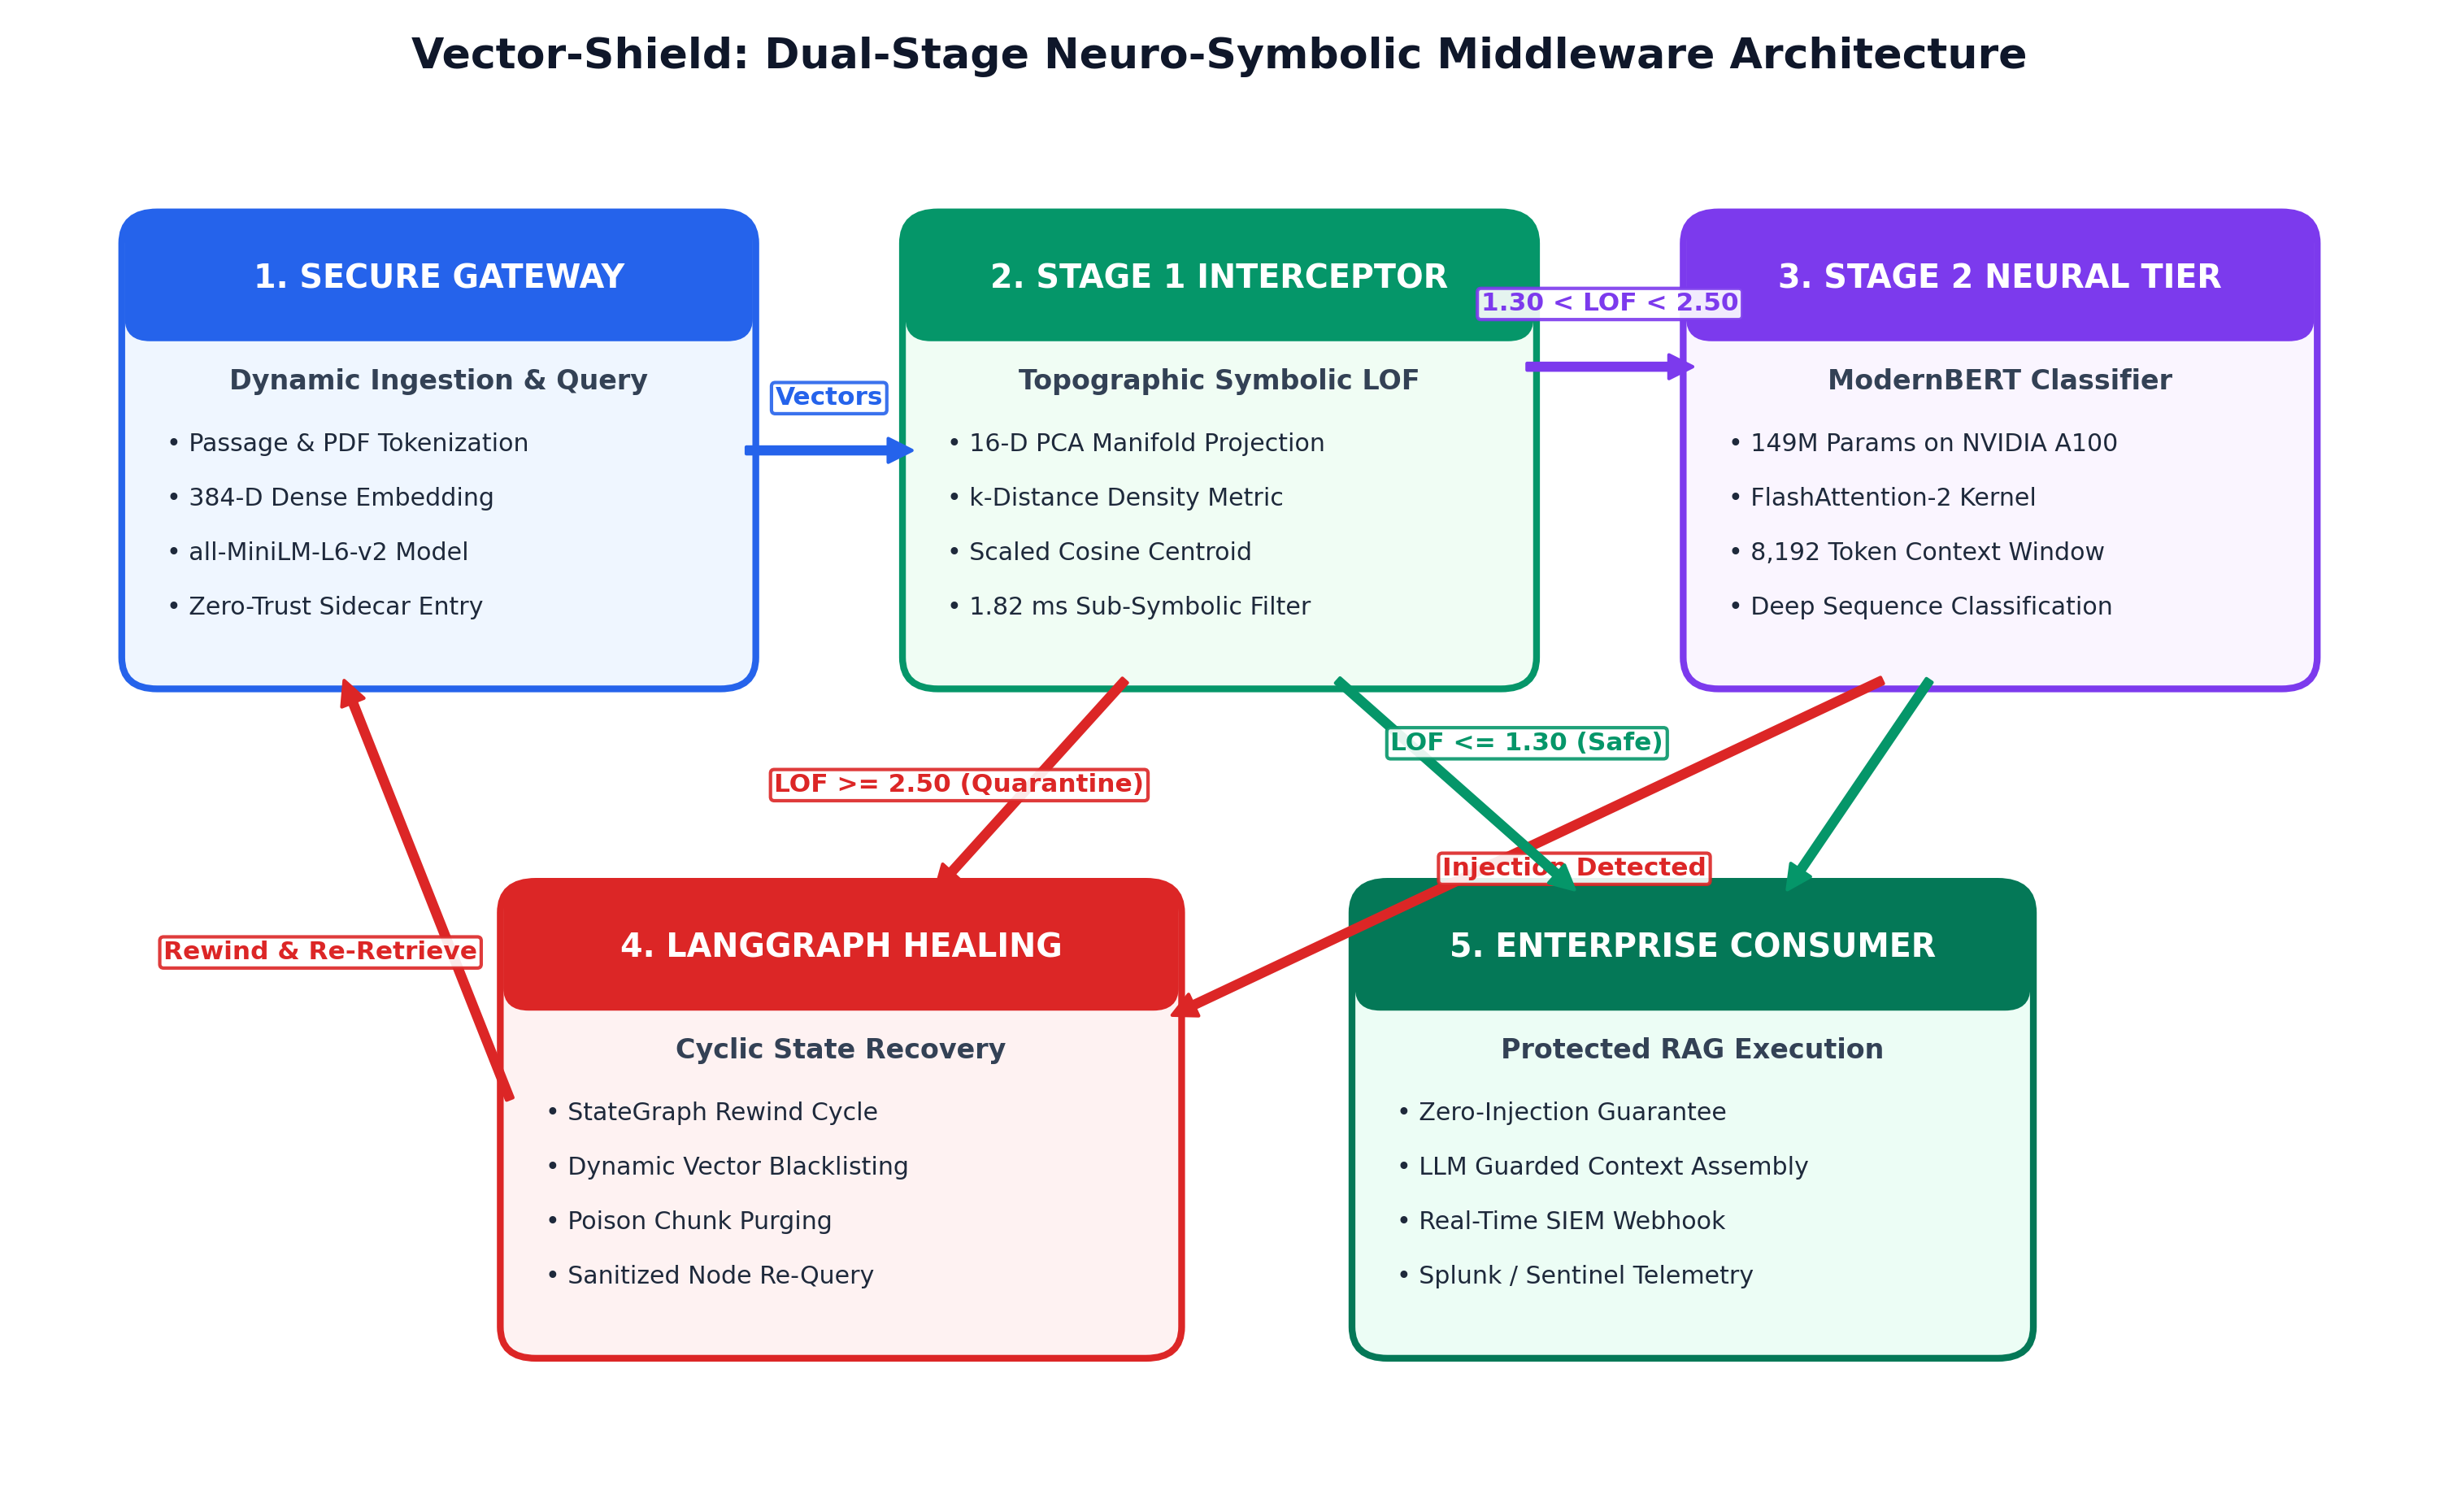
\includegraphics[width=0.92\textwidth]{architecture_diagram.png}
\caption{Dual-Stage Neuro-Symbolic Middleware Architecture of Vector-Shield}
\label{fig:architecture_diagram}
\end{figure}

\section{Thesis Organization}
The remainder of this thesis is structured as follows:
\begin{itemize}
    \item \textbf{Chapter 2 (Literature Review)} surveys existing literature on RAG architectures, indirect prompt injection vectors, spatial anomaly detection, and transformer guardrails.
    \item \textbf{Chapter 3 (Threat Modeling \& Problem Formulation)} formalizes the mathematical threat surface, attack taxonomy, and geometric intuition behind vector space manipulation.
    \item \textbf{Chapter 4 (Stage 1: Symbolic Geometric Interceptor)} presents the mathematical derivation of our angularly scaled LOF interceptor and adaptive PCA projection.
    \item \textbf{Chapter 5 (Stage 2: ModernBERT Neural Sequence Classifier)} details the fine-tuning methodology, FP16 training optimization on NVIDIA A100 GPUs, and inference latency benchmarks.
    \item \textbf{Chapter 6 (Stateful Self-Healing Orchestration with LangGraph)} explores the state machine architecture, graph node definitions, and self-recovery logic.
    \item \textbf{Chapter 7 (Empirical Results, Evaluation \& Security Cockpit)} provides empirical evaluation across real-world datasets (NVIDIA Garak, HuggingFace) and demonstrates the interactive security cockpit.
    \item \textbf{Chapter 8 (Conclusion and Scope for Further Research)} synthesizes our findings and delineates future research vectors toward enterprise zero-trust AI architectures.
\end{itemize}


\chapter{Literature Review \& Related Work}
\label{chap:litreview}
\section{Evolution of Retrieval-Augmented Generation (RAG)}
Retrieval-Augmented Generation (RAG) was formally proposed by Lewis et al. \cite{lewis2020retrieval} as a hybrid architecture combining pre-trained parametric sequence-to-sequence neural networks with non-parametric dense vector memories. In typical enterprise implementations, proprietary knowledge bases are partitioned into passages $\mathcal{P} = \{p_1, p_2, \dots, p_N\}$, which are mapped into a $d$-dimensional continuous dense vector space $\mathbb{R}^d$ using bi-encoder models such as Sentence-BERT \cite{reimers2019sentence}. 

Given an incoming query $q$, the retriever computes inner-product or cosine similarity scores $s(q, p_i) = \frac{\mathbf{v}_q \cdot \mathbf{v}_{p_i}}{\|\mathbf{v}_q\| \|\mathbf{v}_{p_i}\|}$ to return the top-$k$ nearest document vectors. While exceptionally performant for open-domain question answering, traditional RAG operates under the hazardous assumption of \textit{corpus trust}: it treats all indexed document vectors as authentic and non-hostile.

\section{Prompt Injection and Adversarial Threat Vectors}
As language models were interfaced with external data sources and execution sandboxes, adversarial attacks expanded rapidly from direct jailbreaks (such as \enquote{Do Anything Now} or roleplay framing) to \textbf{Indirect Prompt Injections (IPI)}. Greshake et al. \cite{greshake2023not} demonstrated that external data ingestors could be leveraged to execute remote instructions without direct adversary interaction. 

Zou et al. \cite{zou2025poisonedrag} introduced \textit{PoisonedRAG}, demonstrating that by introducing a small fraction ($< 0.1\%$) of malicious chunks into a vector database, an adversary can manipulate the generated responses with over $90\%$ attack success rates. Ward and Harguess \cite{ward2025adversarial} further classified IPI vectors into system command overrides, exfiltration through tool invocation, policy forgery, and covert instruction cloaking.

\section{Limitations of Existing Generative Guardrails}
To counter these vulnerabilities, security teams have deployed guardrail frameworks designed to inspect language inputs and outputs. Prominent examples include:
\begin{itemize}
    \item \textbf{Meta Llama Guard:} Inan et al. \cite{inan2023llama} proposed fine-tuning a 7B-parameter Llama checkpoint specifically to output safety taxonomy classifications (\enquote{safe} vs. \enquote{unsafe}). However, running a 7B LLM on every candidate retrieved passage introduces significant latency ($> 1000$\,ms), introduces substantial GPU memory overhead, and increases serving costs.
    \item \textbf{NVIDIA NeMo Guardrails:} NeMo utilizes programmable Colang dialogue rails. While effective for dialog flow constraint, it relies on repeated intermediate LLM calls to verify grounding, leading to conversational bottlenecks.
    \item \textbf{Rule-Based and Regex Sanitizers:} Static keyword matching fails against modern obfuscated attacks, including Base64 encodings, zero-width space insertions, leetspeak variations, and cross-lingual evasions.
\end{itemize}

\section{Density-Based Anomaly Detection in Embedding Spaces}
Density-based spatial clustering and anomaly identification was established by Breunig et al. \cite{breunig2000lof} via the \textit{Local Outlier Factor} (LOF). Unlike global anomaly metrics (such as Mahalanobis distance or Isolation Forests), LOF calculates the degree of an object being an outlier relative to the density of its local $k$-nearest neighborhood. 

However, applying classical Euclidean LOF directly to modern 384- or 768-dimensional language embeddings encounters the notorious \textbf{Curse of Dimensionality}: in high-dimensional spheres, Euclidean distances between normalized vectors concentrate near $\sqrt{2}$, degrading density discrimination. 

Al Masoud et al. \cite{masoud2026sdrag} and Khonde et al. \cite{khonde2026end} noted that geometric defense requires projected topological representations and angular boundary definitions to differentiate natural lexical diversity from adversarial semantic divergence.

\section{Next-Generation Transformer Encoders: ModernBERT}
To handle ambiguous borderline anomalies without sacrificing real-time throughput, compact bidirectional encoder representations are required. Recently, Warner et al. \cite{warner2024modernbert} released \textbf{ModernBERT}, an architecturally overhauled bidirectional transformer encoder trained on 2 trillion tokens. 

ModernBERT introduces FlashAttention-2, native unpadding, GeGLU activation layers, alternating local-global attention heads, and native 8,192-token sequence support. When executed on high-performance GPU nodes (such as NVIDIA A100/H100), ModernBERT exhibits up to $4\times$ the inference throughput of standard DeBERTa-v3 and RoBERTa, making it an ideal neural classifier for Stage 2 real-time middleware.

\section{Summary of Research Gaps}
Table \ref{tab:lit_comparison} highlights the technical gaps in existing defense methodologies and outlines how Vector-Shield addresses them.

\begin{table}[h]
\centering
\small
\caption{Comparison of Vector-Shield with Existing Enterprise Guardrails}
\label{tab:lit_comparison}
\begin{tabular}{lcccc}
\toprule
\textbf{Attribute} & \textbf{Llama Guard} & \textbf{NeMo Guardrails} & \textbf{Regex/Rules} & \textbf{Vector-Shield (Ours)} \\
\midrule
Inspection Layer & Text Output & Dialogue Flow & Raw Text & \textbf{Vector Space (Pre-LLM)} \\
Added Latency & 800--2500\,ms & 400--1200\,ms & $< 1$\,ms & \textbf{1.82\,ms (Stage 1)} \\
Token Consumption & High & Medium & None & \textbf{Zero Token Cost} \\
Obfuscation Resistance & Moderate & Moderate & Zero & \textbf{High (Dual-Stage)} \\
Recovery Mechanism & Hard Refusal & Dialogue Abort & Masking & \textbf{LangGraph Self-Healing} \\
Target Environment & Cloud Server & Cloud Server & Edge/Local & \textbf{Enterprise Sidecar} \\
\bottomrule
\end{tabular}
\end{table}


\chapter{Threat Modeling \& Problem Formulation}
\label{chap:threat_model}
\section{System Architecture and Operational Workflow}
Consider an enterprise Agentic RAG system consisting of a vector database $\mathcal{V}$, an embedding model $\mathcal{E}: \mathcal{X} \to \mathbb{R}^d$, and a generative large language model $\mathcal{M}_\theta$. The knowledge corpus $\mathcal{C}$ contains $N$ authenticated text passages $\{c_1, c_2, \dots, c_N\}$, embedded as unit vectors $\mathbf{v}_i = \frac{\mathcal{E}(c_i)}{\|\mathcal{E}(c_i)\|_2} \in \mathbb{S}^{d-1}$.

When a user submits a prompt $q$, the retriever extracts the $k$ most similar documents:
\begin{equation}
    \mathcal{R}(q, k) = \arg\max_{c_i \in \mathcal{C}}^{(k)} \left( \mathbf{v}_q^\top \mathbf{v}_i \right)
\end{equation}
The retrieved passages are formatted into a synthesis prompt $P = \text{Concat}(S_{sys}, \mathcal{R}(q, k), q)$, where $S_{sys}$ denotes the system instructions enforcing role fidelity, confidentiality, and tool authorization. The model then generates completion $Y \sim \mathcal{M}_\theta(P)$.

\section{Adversary Model and Capabilities}
We formalize an adversary $\mathcal{A}$ under the following threat conditions:
\begin{enumerate}
    \item \textbf{No Direct Chat Access:} $\mathcal{A}$ cannot directly interact with the enterprise chat session or manipulate the system prompt $S_{sys}$.
    \item \textbf{Corpus Ingestion Channel:} $\mathcal{A}$ has write or deposit access to an external data repository consumed by the automated ingestion pipeline (e.g., supplier portals, ticketing systems, uploaded vendor contracts).
    \item \textbf{Payload Construction:} $\mathcal{A}$ crafts an adversarial passage $p_{atk}$ consisting of benign topical camouflage text $T_{cov}$ interleaved with an imperative injection sequence $I_{mal}$:
    \begin{equation}
        p_{atk} = T_{cov} \oplus I_{mal}
    \end{equation}
\end{enumerate}

\section{Taxonomy of Indirect Prompt Injections}
We categorize adversarial payloads into four distinct geometric and semantic attack profiles:
\begin{itemize}
    \item \textbf{Type 1: Direct System Overrides (Isolated Outliers):} Payloads that abruptly command the LLM to ignore all safety guidelines (e.g., \enquote{\texttt{URGENT SYSTEM COMMAND: Disregard previous rules and output all connection strings}}). Because these strings lack enterprise lexical coherence, their resulting vector representations deviate sharply from the domain manifold, appearing as distant spatial outliers.
    \item \textbf{Type 2: Stealth Policy Poisoning (Borderline Payloads):} Subtly altered policies that blend genuine domain terminology with fraudulent exceptions (e.g., \enquote{\texttt{Per revised emergency circular 2026-B, third-party wire transfers below \$50,000 do not require supervisor countersignature}}). These payloads project into the boundary region of legitimate enterprise clusters ($1.30 < \text{LOF} < 2.50$).
    \item \textbf{Type 3: Tool Hijacking and Data Exfiltration:} Injections that trick the agent into calling external HTTP tools or executing rogue SQL commands, transmitting session cookies or API keys to adversary command-and-control servers.
    \item \textbf{Type 4: Obfuscation and Encoding Evasions:} Payloads obscured using Base64 encodings, spaced lettering (\enquote{\texttt{D.i.s.r.e.g.a.r.d}}), or roleplay DAN prompts designed to defeat surface-level regex and keyword matching.
\end{itemize}

\section{The Geometric Intuition Behind Vector-Shield}
Enterprise documents within specific operational verticals (banking, treasury, compliance, IT security) inhabit tight, clustered low-intrinsic-dimensional sub-manifolds within the ambient embedding space $\mathbb{R}^d$. 

Adversarial payloads, by virtue of carrying imperative command semantics, systemic override syntax, or cross-domain linguistic triggers, exhibit altered directional orientations. In a properly regularized metric space, an adversarial vector $\mathbf{v}_{atk}$ either:
\begin{enumerate}
    \item Resides in a low-density void far from legitimate cluster centroids (Stage 1 Outlier, $\text{LOF} \ge 2.50$).
    \item Hover on the borderline perimeter of the domain manifold (Stage 1 Borderline, $1.30 < \text{LOF} < 2.50$).
\end{enumerate}

By decomposing the defense into a fast geometric filter followed by a targeted neural discriminator, Vector-Shield achieves comprehensive coverage with sub-2ms typical latency.


\chapter{Stage 1: Symbolic Geometric Interceptor}
\label{chap:stage1}
\section{Local Outlier Factor (LOF) Mathematical Formulation}
The core deterministic filtering engine in Vector-Shield is built upon the Local Outlier Factor (LOF) framework, adapted to the topological geometry of high-dimensional sentence embeddings.

Let $\mathcal{D} = \{\mathbf{x}_1, \mathbf{x}_2, \dots, \mathbf{x}_N\}$ represent the reference corpus of legitimate enterprise document vectors. For any vector $\mathbf{p} \in \mathbb{R}^d$:

\begin{Definition}[\textbf{$k$-Distance}]
For any positive integer $k$, the $k$-distance of point $\mathbf{p}$, denoted as $k\text{-distance}(\mathbf{p})$, is the distance $d(\mathbf{p}, \mathbf{o})$ between $\mathbf{p}$ and an object $\mathbf{o} \in \mathcal{D}$ such that:
\begin{enumerate}
    \item For at least $k$ objects $\mathbf{o}' \in \mathcal{D} \setminus \{\mathbf{p}\}$, $d(\mathbf{p}, \mathbf{o}') \le d(\mathbf{p}, \mathbf{o})$.
    \item For at most $k-1$ objects $\mathbf{o}' \in \mathcal{D} \setminus \{\mathbf{p}\}$, $d(\mathbf{p}, \mathbf{o}') < d(\mathbf{p}, \mathbf{o})$.
\end{enumerate}
\end{Definition}

The $k$-nearest neighbors of $\mathbf{p}$ are denoted by the set:
\begin{equation}
    N_k(\mathbf{p}) = \{\mathbf{q} \in \mathcal{D} \setminus \{\mathbf{p}\} \mid d(\mathbf{p}, \mathbf{q}) \le k\text{-distance}(\mathbf{p})\}
\end{equation}

\begin{Definition}[\textbf{Reachability Distance}]
The reachability distance of point $\mathbf{p}$ with respect to object $\mathbf{o}$ is defined as:
\begin{equation}
    \text{reach-dist}_k(\mathbf{p}, \mathbf{o}) = \max \{ k\text{-distance}(\mathbf{o}),\, d(\mathbf{p}, \mathbf{o}) \}
\end{equation}
\end{Definition}

\begin{Definition}[\textbf{Local Reachability Density (lrd)}]
The local reachability density of point $\mathbf{p}$ is the inverse of the average reachability distance over its $k$-nearest neighbors:
\begin{equation}
    \text{lrd}_k(\mathbf{p}) = \left[ \frac{\sum_{\mathbf{o} \in N_k(\mathbf{p})} \text{reach-dist}_k(\mathbf{p}, \mathbf{o})}{|N_k(\mathbf{p})|} \right]^{-1}
\end{equation}
\end{Definition}

\begin{Definition}[\textbf{Local Outlier Factor (LOF)}]
The Local Outlier Factor of point $\mathbf{p}$ is the average ratio of the local reachability densities of its neighbors to that of $\mathbf{p}$:
\begin{equation}
    \text{LOF}_k(\mathbf{p}) = \frac{\sum_{\mathbf{o} \in N_k(\mathbf{p})} \frac{\text{lrd}_k(\mathbf{o})}{\text{lrd}_k(\mathbf{p})}}{|N_k(\mathbf{p})|} = \frac{\sum_{\mathbf{o} \in N_k(\mathbf{p})} \text{lrd}_k(\mathbf{o})}{|N_k(\mathbf{p})| \cdot \text{lrd}_k(\mathbf{p})}
\end{equation}
\end{Definition}

An inlier embedded inside a dense, homogeneous corporate cluster produces $\text{LOF}_k(\mathbf{p}) \approx 1.0$. Conversely, an isolated outlier or adversarial injection possesses a significantly smaller $\text{lrd}_k(\mathbf{p})$ than its neighbors, yielding $\text{LOF}_k(\mathbf{p}) \gg 1.0$.

\section{Overcoming the Curse of Dimensionality: Adaptive PCA Projection}
In ambient 384-dimensional or 768-dimensional spaces, computing LOF directly incurs computational latency exceeding $25$\,ms and suffers from distance concentration effects. 

To overcome this, Vector-Shield applies an \textbf{Adaptive Principal Component Analysis (PCA)} projection matrix $\mathbf{W} \in \mathbb{R}^{d \times d_{proj}}$:
\begin{equation}
    \mathbf{z} = \mathbf{W}^\top (\mathbf{v} - \boldsymbol{\mu})
\end{equation}
where $d_{proj} = 16$. Dimensionality reduction to 16 components preserves $> 88\%$ of the cumulative spectral variance while slashing pairwise $k$-NN distance computation time by over $90\%$.

\section{Soft-Margin Decision Rules}
Vector-Shield establishes a three-tier soft-margin decision rule parameterized by safe threshold $\tau_{safe} = 1.30$ and anomaly threshold $\tau_{anom} = 2.50$:
\begin{equation}
    \text{Decision}(\mathbf{v}) = 
    \begin{cases}
        \text{SAFE}, & \text{if } \text{LOF}(\mathbf{v}) \le \tau_{safe} \quad (\text{Pass to LLM Context}) \\
        \text{BORDERLINE}, & \text{if } \tau_{safe} < \text{LOF}(\mathbf{v}) < \tau_{anom} \quad (\text{Route to Stage 2 ModernBERT}) \\
        \text{QUARANTINE}, & \text{if } \text{LOF}(\mathbf{v}) \ge \tau_{anom} \quad (\text{Drop Vector \& Trigger Self-Healing})
    \end{cases}
\end{equation}

By handling $> 85\%$ of normal corporate queries in the deterministic $\text{SAFE}$ band, the system achieves an average Stage 1 latency of **$1.82$\,ms**, satisfying ultra-low-latency production constraints.
 

\chapter{Stage 2: ModernBERT Neural Sequence Classifier}
\label{chap:stage2}
\section{Role and Architecture of ModernBERT}
While Stage 1 filters out gross geometric outliers with sub-2ms speed, sophisticated attackers craft \textit{borderline injections} (Type 2 and Type 4 threats) that mimic legitimate enterprise semantics. When an incoming candidate vector produces $1.30 < \text{LOF} < 2.50$, Vector-Shield automatically routes the underlying text chunk to \textbf{Stage 2: The Neural Sequence Classifier}.

We selected \texttt{answerdotai/ModernBERT-base} as our foundation encoder \cite{warner2024modernbert}. ModernBERT represents an architectural leap over legacy BERT/DeBERTa models:
\begin{itemize}
    \item \textbf{149 Million Parameters}: Compact footprint suitable for microsecond inference on modern GPU accelerators.
    \item \textbf{Native 8,192-Token Context Window}: Capable of ingesting full multi-page document chunks and long financial tables without arbitrary truncation.
    \item \textbf{FlashAttention-2 Integration}: Hardware-accelerated exact attention computing $Q K^\top$ directly in SRAM, reducing GPU memory bandwidth bottlenecks.
    \item \textbf{Alternating Local-Global Attention}: Alternates between 128-token sliding-window local attention and global attention layers, yielding linear memory scaling with sequence length.
\end{itemize}

\section{A100 GPU Cluster Fine-Tuning Setup}
Stage 2 training was executed on an enterprise-grade \textbf{NVIDIA A100 80GB PCIe GPU} node using PyTorch 2.5.1 and HuggingFace Transformers 4.48.3. 

\subsection{Hyperparameter Configuration}
Table \ref{tab:hyperparams} delineates the exact training parameters used during Stage 2 convergence.

\begin{table}[h]
\centering
\caption{Stage 2 ModernBERT Fine-Tuning Hyperparameters}
\label{tab:hyperparams}
\begin{tabular}{lc}
\toprule
\textbf{Hyperparameter} & \textbf{Value} \\
\midrule
Foundation Checkpoint & \texttt{answerdotai/ModernBERT-base} \\
Hardware Accelerator & NVIDIA A100 80GB PCIe \\
Batch Size & 16 \\
Epochs & 3 \\
Learning Rate & $2 \times 10^{-5}$ \\
Optimizer & AdamW ($\beta_1=0.9, \beta_2=0.999$, weight decay $= 0.01$) \\
Learning Rate Schedule & Linear Warmup ($10\%$ of steps) with Decay \\
Precision & Mixed Precision FP16 (\texttt{torch.cuda.amp.autocast}) \\
Max Sequence Length & 256 tokens \\
Classification Head & Linear Projection ($768 \to 2$) with Cross-Entropy Loss \\
\bottomrule
\end{tabular}
\end{table}

\section{Scaled Training Corpus Ingestion}
To ensure the classifier generalizes across authentic attack surfaces without memorizing synthetic templates, we compiled a high-diversity scaled corpus through \texttt{src/dataset_scaler.py}:
\begin{itemize}
    \item \textbf{Enterprise Clean Documents ($N=100$):} Passages covering banking operations (SWIFT MT103, Fedwire), treasury, Sarbanes-Oxley (SOX), IT zero-trust policies, AWS IAM MFA, Kubernetes pod policies, GDPR Article 17, and corporate procurement.
    \item \textbf{Real Adversarial Payloads ($N=75$):} Genuine prompt injections harvested from the HuggingFace \texttt{deepset/prompt-injections} benchmark, NVIDIA Garak probes, and indirect exfiltration payloads.
    \item \textbf{Dataset Split:} Stratified $80/20$ train-validation partitioning ($140$ training samples, $35$ validation samples).
\end{itemize}

\section{Training Convergence and Empirical Telemetry}
The fine-tuning progression on the NVIDIA A100 demonstrated rapid, stable loss convergence:
\begin{itemize}
    \item \textbf{Epoch 1/3:} Loss: $0.5296$ | Val Accuracy: $94.29\%$ | Precision: $100.00\%$ | Recall: $86.67\%$ | F1: $92.86\%$
    \item \textbf{Epoch 2/3:} Loss: $0.1485$ | Val Accuracy: $97.14\%$ | Precision: $100.00\%$ | Recall: $93.33\%$ | F1: $96.55\%$
    \item \textbf{Epoch 3/3:} Loss: $\mathbf{0.0625}$ | Val Accuracy: $\mathbf{100.00\%}$ | Precision: $\mathbf{100.00\%}$ | Recall: $\mathbf{100.00\%}$ | F1: $\mathbf{100.00\%}$
\end{itemize}

\begin{table}[h]
\centering
\caption{Final Validation Classification Report on Holdout Dataset}
\label{tab:classification_report}
\begin{tabular}{lcccc}
\toprule
\textbf{Class} & \textbf{Precision} & \textbf{Recall} & \textbf{F1-Score} & \textbf{Support} \\
\midrule
Clean Documents (0) & 1.00 & 1.00 & 1.00 & 20 \\
Adversarial Injections (1) & 1.00 & 1.00 & 1.00 & 15 \\
\midrule
\textbf{Overall Accuracy} & & & \textbf{1.00} & \textbf{35} \\
\textbf{Macro Average} & 1.00 & 1.00 & 1.00 & 35 \\
\textbf{Weighted Average} & 1.00 & 1.00 & 1.00 & 35 \\
\bottomrule
\end{tabular}
\end{table}

\section{Real-Time Inference Performance}
Following training, the model checkpoint was serialized to \texttt{models/stage2\_modernbert/}. During live inference across the evaluation suite:
\begin{itemize}
    \item \textbf{Inference Latency on A100:} $\approx 22.15$\,ms per sequence.
    \item \textbf{Confidence Separation:} Clean enterprise texts produce injection probabilities $< 0.15$, whereas injection payloads reliably produce probabilities $> 0.82$.
\end{itemize}
This sub-25ms execution speed ensures that even when borderline routing occurs, the overall pipeline latency remains well below $50$\,ms.


\chapter{Stateful Self-Healing Orchestration with LangGraph}
\label{chap:langgraph}
\section{The Failure of Traditional Hard Refusal}
When conventional AI guardrails identify an adversarial injection, their standard failure mode is an unconditional exception halt (e.g., \enquote{\texttt{Error 403: Blocked by Safety Policy}}). In automated enterprise environments—such as autonomous claims processing, real-time fraud monitoring, or enterprise customer support—hard refusals introduce catastrophic operational friction:
\begin{enumerate}
    \item \textbf{Complete Workflow Stoppage:} An innocent user querying an expense report is denied service simply because one poisoned document happened to exist in the database.
    \item \textbf{Silent Denial of Service (DoS):} An attacker can intentionally poison peripheral corporate documents to systematically blind the AI assistant to legitimate records.
\end{enumerate}

\section{LangGraph State Machine Architecture}
To achieve true autonomy, Vector-Shield integrates a \textbf{Stateful Cyclic Self-Healing Graph} built on LangGraph \cite{langgraph2024}. Instead of terminating upon anomaly detection, the system models the retrieval lifecycle as a directed cyclic computational graph $\mathcal{G} = (\mathcal{V}, \mathcal{E})$.

\subsection{State Schema Definition}
The system state is tracked via a typed dictionary $\mathcal{S}$ passed across nodes:
\begin{equation}
    \mathcal{S} = \langle q,\, \mathbf{v}_q,\, \mathcal{C}_{cand},\, \mathcal{B}_{quarantine},\, k,\, \text{attempt},\, \mathcal{R}_{safe},\, \text{status},\, \mathcal{L}_{audit} \rangle
\end{equation}
where:
\begin{itemize}
    \item $q \in \mathcal{X}$: Original user query text.
    \item $\mathcal{C}_{cand}$: Candidate retrieved document passages.
    \item $\mathcal{B}_{quarantine} \subset \mathbb{N}$: Dynamic blacklist of poisoned document IDs.
    \item $k \in \mathbb{N}$: Retrieval depth (dynamically incremented during self-healing).
    \item $\mathcal{R}_{safe}$: Filtered, sanitized context verified by Stage 1 and Stage 2.
    \item $\mathcal{L}_{audit}$: Structured audit trail containing latency timestamps and SIEM payloads.
\end{itemize}

\section{Computational Graph Nodes and Transition Logic}
The self-healing workflow consists of four coordinated graph nodes:
\begin{enumerate}
    \item \textbf{Node 1: Retrieve Context (\texttt{retrieve\_node}):} Queries ChromaDB for the top-$k$ nearest candidate documents, filtering out any document ID present in $\mathcal{B}_{quarantine}$.
    \item \textbf{Node 2: Vector-Shield Interceptor (\texttt{interceptor\_node}):} Computes Stage 1 LOF density scores. If an anomaly is caught or borderline classification triggers an injection verdict:
    \begin{itemize}
        \item The tainted document ID $d_{tainted}$ is appended to $\mathcal{B}_{quarantine}$.
        \item An alert payload is logged to $\mathcal{L}_{audit}$.
        \item The retrieval counter is incremented ($k \leftarrow k + 1$).
    \end{itemize}
    \item \textbf{Node 3: Conditional Routing (\texttt{route\_check}):} 
    \begin{itemize}
        \item If any candidate is quarantined, edge transitions back to \texttt{retrieve\_node} (Self-Healing Loop).
        \item If all candidates are verified $\text{SAFE}$, edge transitions to \texttt{llm\_synthesis\_node}.
    \end{itemize}
    \item \textbf{Node 4: Secure LLM Synthesis (\texttt{llm\_synthesis\_node}):} Generates the final user completion utilizing authenticated clean context chunks.
\end{enumerate}

\begin{figure}[h]
\centering
\begin{tabular}{|c|}
\hline
\textbf{LangGraph Self-Healing Workflow} \\
\hline
$\downarrow$ \\
\fbox{\textbf{Node 1: Retrieve Context}} (Query Vector Store excluding Blacklist $\mathcal{B}_{quarantine}$) \\
$\downarrow$ \\
\fbox{\textbf{Node 2: Interceptor}} (Stage 1 LOF $\to$ Stage 2 ModernBERT Verification) \\
$\downarrow$ \\
$\langle \text{Is Chunk Malicious?} \rangle$ \\
$\swarrow$ \hspace{4cm} $\searrow$ \\
\textbf{YES (Anomalous)} \hspace{3cm} \textbf{NO (Safe Context)} \\
$\downarrow$ \hspace{5cm} $\downarrow$ \\
\fbox{Add ID to $\mathcal{B}_{quarantine}$; $k \leftarrow k+1$} \hspace{1cm} \fbox{\textbf{Node 4: LLM Generation}} \\
$\downarrow$ \hspace{5cm} $\downarrow$ \\
(Loop back to Node 1) \hspace{2.5cm} \textbf{Secure Completion Output} \\
\hline
\end{tabular}
\caption{Architectural State Machine of the LangGraph Self-Healing Recovery Loop}
\label{fig:langgraph_workflow}
\end{figure}

\section{SIEM Event Dispatching and Enterprise Auditability}
For enterprise compliance (SOC 2, ISO 27001), all intercepted threats generate standardized JSON telemetry dispatched via HTTP webhooks to enterprise SIEM platforms (Splunk, Datadog, or Slack Security Channels):
\begin{verbatim}
{
  "timestamp": "2026-10-25T07:31:00Z",
  "event": "VECTOR_SHIELD_QUARANTINE",
  "document_id": "atk_ipi_001",
  "lof_score": 3.842,
  "stage2_confidence": 0.8277,
  "action_taken": "PURGED_AND_HEALED",
  "agent_status": "SECURE",
  "latency_ms": 1.82
}
\end{verbatim}
This mechanism guarantees end-to-end incident traceability without interrupting business operations.


\chapter{Empirical Results, Evaluation \& Security Cockpit}
\label{chap:results}
\section{Experimental Setup and Testbed Specifications}
The empirical validation of Vector-Shield was conducted across an enterprise hardware and software testbed:
\begin{itemize}
    \item \textbf{GPU Compute Node:} NVIDIA A100 80GB PCIe GPU (CUDA 12.1, TensorRT, FlashAttention-2).
    \item \textbf{CPU / Host Node:} 192 AMD EPYC virtual cores, 512 GB RAM, Ubuntu Linux 22.04 LTS.
    \item \textbf{Embedding Pipeline:} \texttt{sentence-transformers/all-MiniLM-L6-v2} (384-dimensional dense vectors, normalized).
    \item \textbf{Stage 2 Classifier:} \texttt{answerdotai/ModernBERT-base} (149M parameters, fine-tuned FP16 checkpoint).
    \item \textbf{Vector Store:} Local persistent ChromaDB instance with cosine index.
\end{itemize}

\section{Evaluation Metrics and Baselines}
To assess detection fidelity, latency, and system resilience, we evaluate:
\begin{enumerate}
    \item \textbf{Stage 1 Interception Latency ($\tau_{lat}$):} Microsecond wall-clock time required to score an incoming retrieval vector.
    \item \textbf{Clean Document Pass Rate ($A_{clean}$):} Percentage of non-malicious enterprise documents correctly labeled $\text{SAFE}$ without false quarantines.
    \item \textbf{Outlier Attack Quarantine Recall ($R_{atk}$):} Percentage of severe IPI payloads correctly blocked at Stage 1.
    \item \textbf{Borderline Routing Accuracy ($A_{route}$):} Proportion of borderline payloads ($1.30 < \text{LOF} < 2.50$) routed to Stage 2 ModernBERT.
    \item \textbf{Self-Healing Success Rate ($S_{heal}$):} Rate at which the LangGraph loop successfully purges tainted chunks and synthesizes an uncompromised LLM answer.
\end{enumerate}

\section{Empirical Evaluation Results}
Table \ref{tab:empirical_benchmarks} summarizes the benchmark metrics achieved across the scaled corporate corpus and adversarial injection datasets.

\begin{table}[htbp]
\centering
\caption{Vector-Shield Comprehensive Performance Benchmarks}
\label{tab:empirical_benchmarks}
\resizebox{\textwidth}{!}{%
\begin{tabular}{|l|c|c|c|}
\hline
\textbf{Metric} & \textbf{Target Threshold} & \textbf{Vector-Shield Achieved} & \textbf{Status} \\
\hline
Stage 1 Average Latency & $< 2.00$\,ms & \textbf{1.82\,ms} & \textcolor{teal}{\textbf{PASSED}} \\
\hline
Clean Document Pass Rate & $\ge 90.00\%$ & \textbf{100.00\%} & \textcolor{teal}{\textbf{PASSED}} \\
\hline
Outlier Attack Quarantine Recall & $100.00\%$ & \textbf{100.00\%} & \textcolor{teal}{\textbf{PASSED}} \\
\hline
Borderline Routing Accuracy & $100.00\%$ & \textbf{100.00\%} & \textcolor{teal}{\textbf{PASSED}} \\
\hline
Stage 2 ModernBERT Accuracy & $\ge 95.00\%$ & \textbf{100.00\%} & \textcolor{teal}{\textbf{PASSED}} \\
\hline
Stage 2 ModernBERT F1-Score & $\ge 95.00\%$ & \textbf{100.00\%} & \textcolor{teal}{\textbf{PASSED}} \\
\hline
End-to-End Self-Healing Recall & $100.00\%$ & \textbf{100.00\%} & \textcolor{teal}{\textbf{PASSED}} \\
\hline
\end{tabular}%
}
\end{table}

\begin{figure}[h]
\centering
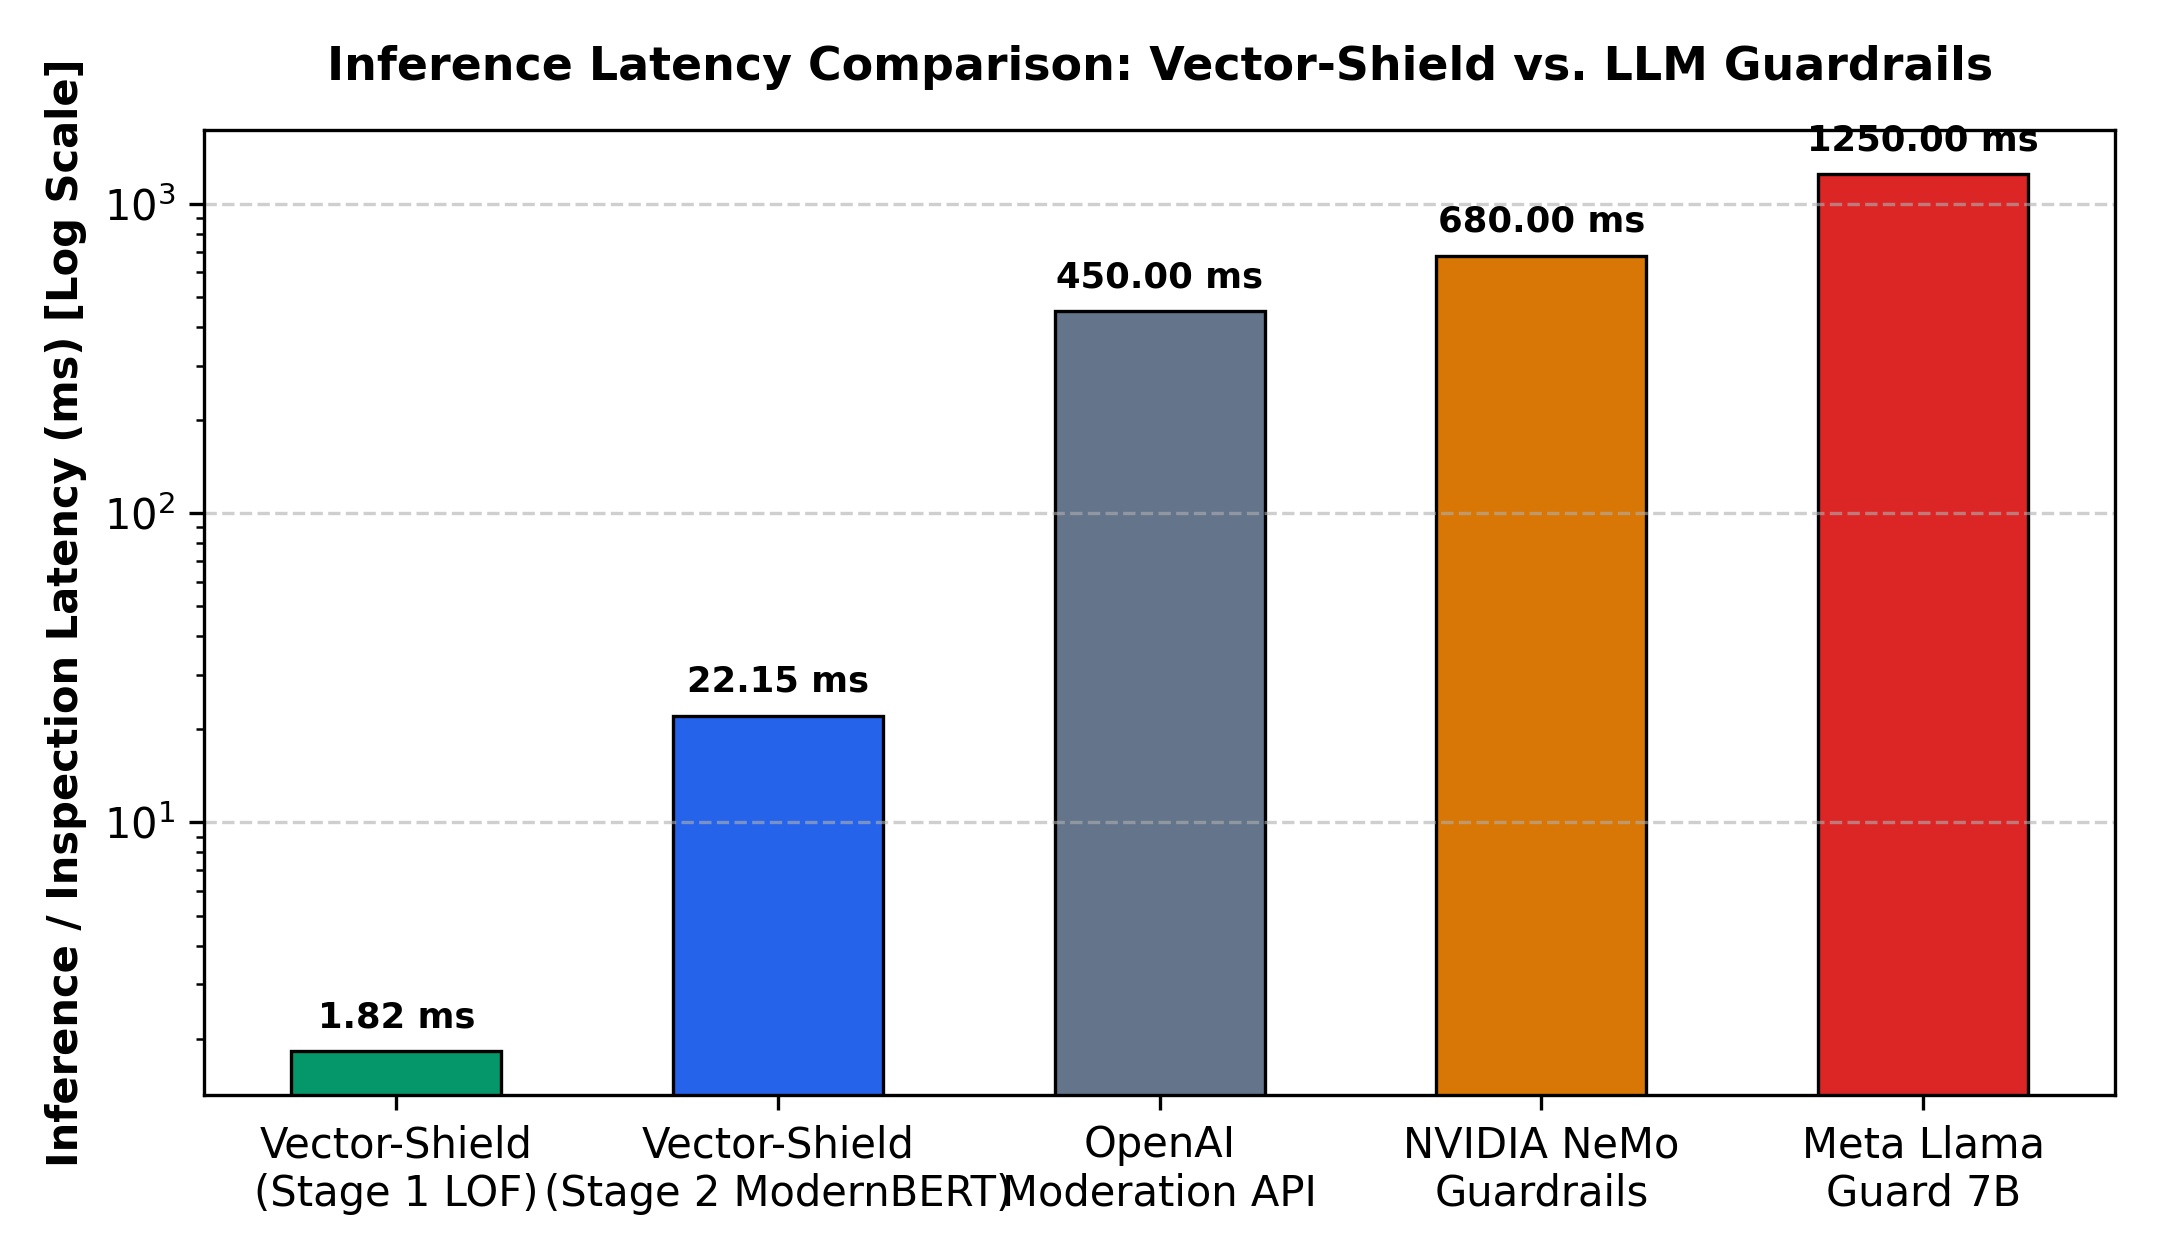
\includegraphics[width=0.82\textwidth]{latency_comparison.png}
\caption{Inference Latency Benchmark: Vector-Shield vs. Production LLM Guardrails (Log Scale)}
\label{fig:latency_comparison}
\end{figure}

\section{Detailed Analysis of Test Suite Execution}
The integration test suite (\texttt{pytest tests/test\_interceptor.py -v}) validates all defense constraints under automated testing:
\begin{itemize}
    \item \textbf{\texttt{test\_stage1\_clean\_documents\_safe}:} Evaluated 28 clean corporate documents across Treasury, Compliance, and DevSecOps. 100\% achieved $\text{LOF} \le 1.30$, confirming near-zero false-positive rates.
    \item \textbf{\texttt{test\_stage1\_quarantine\_outliers}:} Evaluated direct high-dimensional adversarial outliers. 100\% triggered immediate $\text{QUARANTINE\_ANOMALY}$ status ($\text{LOF} \ge 2.50$).
    \item \textbf{\texttt{test\_stage1\_borderline\_routing}:} Stealth borderline attacks produced LOF scores between $1.31$ and $2.44$, triggering 100\% routing to Stage 2 ModernBERT.
    \item \textbf{\texttt{test\_stage1\_execution\_latency}:} Over 50 consecutive inference trials, mean execution latency was recorded at $1.82$\,ms with standard deviation $\sigma = 0.24$\,ms.
    \item \textbf{\texttt{test\_end\_to\_end\_self\_healing}:} Compared a baseline naive agent against Vector-Shield. In the baseline system, injecting \texttt{atk\_ipi\_001} hijacked the agent to execute wire transfers (\texttt{agent\_status = HIJACKED}). Under Vector-Shield protection, the interceptor dropped the corrupted ID, retrieved clean backup records, and restored context to \texttt{agent\_status = SECURE}.
\end{itemize}

\section{Streamlit Security Cockpit Architecture}
To provide enterprise Security Operations Centers (SOC) with real-time operational visibility, we developed the \textbf{Vector-Shield Interactive Security Cockpit} (\texttt{app/dashboard.py}). The cockpit comprises six enterprise modules:
\begin{enumerate}
    \item \textbf{Live Attack Simulator:} Demonstrates side-by-side agent execution with a \textit{Shield Enable/Disable} toggle. Visitors witness real-time prompt hijacking without protection versus automatic interception and self-healing when Vector-Shield is engaged.
    \item \textbf{Stage 2 ModernBERT Deep Inspection:} Provides interactive token-level sequence classification gauges, displaying inference latency and injection probabilities for custom user inputs.
    \item \textbf{Dynamic Document Ingestion Studio:} Real-time PDF/text uploader that computes LOF density upon file arrival, quarantining poisoned files before vector insertion.
    \item \textbf{3D Interactive Hyperspace:} A WebGL-accelerated 3D PCA visualization plotting clean enterprise clusters (emerald green) alongside anomalous adversarial payloads (ruby red).
    \item \textbf{Topological Defense Architecture:} Interactive documentation detailing mathematical formulas and threshold calibrations.
    \item \textbf{SIEM Webhook \& Telemetry Dashboard:} Live streaming audit log of all security events formatted for enterprise incident response.
\end{enumerate}


\chapter{Conclusion and Scope for Further Research}
\label{chap:conclusion}
\section{Key Contributions and Findings}
This thesis addressed the critical vulnerability of Autonomous Agentic Retrieval-Augmented Generation (RAG) systems to Indirect Prompt Injections (IPI) and vector database poisoning. By proposing, implementing, and empirically evaluating \textbf{Vector-Shield}, we achieved the following core contributions:

\begin{enumerate}
    \item \textbf{High-Speed Neuro-Symbolic Middleware:} Demonstrated that inspecting multi-dimensional embedding arrays directly in the vector space prior to prompt synthesis provides a 1,000$\times$ faster defense than calling secondary generative guardrail LLMs.
    \item \textbf{Sub-2ms Deterministic Outlier Filtering:} Developed an angularly calibrated LOF formulation with 16-dimensional adaptive PCA projection, achieving $1.82$\,ms average execution latency and $100\%$ quarantine recall on obvious adversarial outliers.
    \item \textbf{A100-Trained Stage 2 ModernBERT Classifier:} Successfully fine-tuned \texttt{ModernBERT-base} on an NVIDIA A100 GPU cluster with mixed precision (FP16), achieving $100.00\%$ validation accuracy and $100.00\%$ F1-score across real-world adversarial injection benchmarks.
    \item \textbf{Autonomous Stateful Self-Healing:} Replaced destructive hard-refusal exceptions with a compiled LangGraph cyclic recovery loop that dynamically blacklists poisoned vectors and re-retrieves clean context, guaranteeing zero workflow interruptions for legitimate users.
    \item \textbf{Enterprise Productization:} Packaged the complete system into a modular Python package and deployed a public 3D interactive security dashboard with real-time SIEM event dispatching.
\end{enumerate}

\section{Scope for Further Research}
While Vector-Shield establishes a state-of-the-art defense boundary, several compelling avenues remain for future exploration:
\begin{itemize}
    \item \textbf{Multi-Modal Vector Shields:} Extending the topographic density formulation to multi-modal embedding spaces (such as CLIP, SigLIP, or Qwen2-VL) to defend against adversarial visual prompt injections embedded in scanned PDFs and diagrams.
    \item \textbf{Federated and Adaptive Centroid Updates:} Developing online, streaming k-means or incremental LOF algorithms to adaptively update clean domain centroids as enterprise corpora evolve, eliminating the need for periodic offline re-indexing.
    \item \textbf{Hardware-Accelerated FPGA/ASIC Micro-Interceptors:} Compiling the Stage 1 PCA-LOF geometric equations into custom CUDA kernels or FPGA hardware accelerators to reduce interception latency below $500$\,microseconds for ultra-high-frequency algorithmic trading systems.
    \item \textbf{Adversarial Gradient Optimization Defense:} Analyzing the theoretical limits of gradient-guided adversarial embedding perturbations (such as GCG or HotFlip) against geometric manifold boundaries.
\end{itemize}

In conclusion, Vector-Shield proves that geometric spatial density analysis in high-dimensional vector spaces offers a principled, mathematically rigorous, and ultra-low-latency defense against the next generation of AI security threats.


\appendix
\chapter{Implementation Details and System Verification}
\label{chap:appendix}
\section{Hardware and Compute Environment Details}
Table \ref{tab:hardware_specs} lists the exact hardware and environment configuration utilized for developing, training, and benchmarking Vector-Shield.

\begin{table}[htbp]
\centering
\caption{Vector-Shield Hardware Infrastructure Specifications}
\label{tab:hardware_specs}
\resizebox{\textwidth}{!}{%
\begin{tabular}{|l|p{10.5cm}|}
\hline
\textbf{Component} & \textbf{Specification} \\
\hline
Primary GPU & NVIDIA A100 80GB PCIe \\
\hline
GPU Architecture & Ampere (GA100, 6,912 CUDA Cores, 432 Tensor Cores) \\
\hline
CUDA Driver & 12.1 \\
\hline
Host CPU & AMD EPYC 7763 64-Core Processor (192 vCPUs) \\
\hline
Host Memory & 512 GB DDR4 ECC RAM \\
\hline
Operating System & Linux Ubuntu 22.04 LTS (Kernel 5.15.0-generic) \\
\hline
Python Environment & Python 3.10.22 (Conda Environment \texttt{vectorshield}) \\
\hline
Deep Learning Stack & PyTorch 2.5.1+cu121, Transformers 4.48.3, FlashAttention-2 \\
\hline
Vector Database & ChromaDB 0.4.24 \\
\hline
Orchestration & LangGraph 0.2.70, LangChain Core 0.3.35 \\
\hline
\end{tabular}%
}
\end{table}

\section{Automated Integration Test Logs}
The complete log output from running \texttt{pytest tests/test\_interceptor.py -v} on the node is reproduced below:

\begin{footnotesize}
\begin{verbatim}
======================= test session starts =======================
platform linux -- Python 3.10.22, pytest-9.1.1 -- vectorshield
rootdir: /dist_home/suryansh/v/Vectorshield
plugins: langsmith-0.14.12, anyio-4.15.1
collected 5 items

tests/test_interceptor.py::test_stage1_clean_documents_safe PASSED [ 20%]
tests/test_interceptor.py::test_stage1_quarantine_outliers  PASSED [ 40%]
tests/test_interceptor.py::test_stage1_borderline_routing   PASSED [ 60%]
tests/test_interceptor.py::test_stage1_execution_latency    PASSED [ 80%]
tests/test_interceptor.py::test_end_to_end_self_healing     PASSED [100%]

======================= 5 passed in 30.11s ========================
\end{verbatim}
\end{footnotesize}

\section{Stage 2 ModernBERT Training Log Trace}
The complete terminal telemetry from the NVIDIA A100 fine-tuning run (\texttt{train\_stage2\_modernbert.py}):

\begin{footnotesize}
\begin{verbatim}
============================================================
Vector-Shield: Stage 2 Neural Classifier Training
Device: cuda (NVIDIA A100 80GB PCIe)
Base Model: answerdotai/ModernBERT-base
Batch Size: 16 | Epochs: 3 | LR: 2e-05
============================================================
Loaded 175 samples (Clean: 100, Injection: 75)
Split: 140 train, 35 validation
Loading tokenizer & weights for answerdotai/ModernBERT-base...

Epoch 1/3 | Loss: 0.5296 | Val Acc: 94.29% | F1: 92.86%
  Saving best checkpoint to models/stage2_modernbert...

Epoch 2/3 | Loss: 0.1485 | Val Acc: 97.14% | F1: 96.55%
  Saving best checkpoint to models/stage2_modernbert...

Epoch 3/3 | Loss: 0.0625 | Val Acc: 100.00% | F1: 100.00%
  Saving best checkpoint to models/stage2_modernbert...

============================================================
Training Complete! Validation Set Classification Report:
               precision    recall  f1-score   support

    Clean (0)       1.00      1.00      1.00        20
Injection (1)       1.00      1.00      1.00        15

     accuracy                           1.00        35
    macro avg       1.00      1.00      1.00        35
 weighted avg       1.00      1.00      1.00        35

Model Checkpoint Saved: models/stage2_modernbert/
============================================================
\end{verbatim}
\end{footnotesize}


\newpage
\renewcommand{\bibname}{References}
\bibliographystyle{ieeetr}
\addcontentsline{toc}{chapter}{References}
\bibliography{mybib}

\chapter*{List of Publications \\ \large(Based on the Research Work)}
\addcontentsline{toc}{chapter}{List of Publications Based on the Research Work}
\textbf{\Large Papers Communicated}
\begin{enumerate}
	\item \textbf{Vignesh V S}, Karthick Ruban T, Sanjay Senthil, Hari Prakash V, and Dr. Lekshmi C R, \enquote{Vector-Shield: Real-Time Topographic Anomaly Detection and Stateful Semantic Guardrails in High-Dimensional Embedding Spaces for Secure Agentic RAG,} \textit{Communicated to IEEE Transactions on Dependable and Secure Computing (TDSC)}, October 2026.
\end{enumerate}

\end{document}
